\section{Vypracování}
\subsection{Point Location Problem}

Point Location Problem patří mezi základní úlohy výpočetní geometrie a v praxi se s ním setkáváme pokaždé, když klikneme myší do interaktivní mapy nebo herního prostředí.
Cílem je pro daný bod P v rovině R efektivně určit, ve které konkrétní oblasti se bod nachází. 

Zatímco triviální řešení hrubou silou by vyžadovalo testování bodu proti každému polygonu zvlášť, pokročilé algoritmy využívají sofistikované datové struktury k tomu, aby odpověď nalezly v logaritmickém čase. 
Tento problém je klíčový pro geografické informační systémy (GIS) a počítačovou grafiku. 
Pro řešení tohoto problému existuje řada algoritmů.

Jednu skupinu tvoří algortimy Half-plane test a Ray Crossing algorithm, které se využívají při řešení s konvexními mnohouhelníky. 
Pro nekonvexní mnohouelníky se využívají algoritmy Ray Crossing a Winding Number.


\subsection{Ray Crossing Algorithm}
Ze zkoumaného bodu $q$ je vyslána polopřímka (paprsek) $r$. 
Zda bod leží uvnitř či vně polygonu závisí na počtu průsečíků ($k$) paprsku $r$ s hranami polygonu $P$.
Zda bod leží v polygonu zjistíme jednoduše vydělením počtu vrcholů dvěma.
Pokud hodnota po dělení je rovna jedné, bod leží uvnitř polygonu.
Pokud je rovna nule, bod neleží v polygonu.
\[
  k \%2 = \begin{cases}
    0 & { q \in P } \\
    \newline
    1 & { q \notin P}
  \end{cases}
\]

Singulárním případem tohoto algoritmu je, když bod $q$ leží na hraně polygonu.
Pro tuto variantu je nutné použít dva paprsky - levostranný a pravostranný a udržovat si počet levostranných a pravostranných průsečíků ($k_l, k_r$). 
Hlavní myšlenkou je, že pokud $q \in P$, pak $k_l \neq k_r $.

\newpage
\textbf{Pseudokód Ray Crossing}

\algnotext{EndFor}
\algnotext{EndIf}
\algnotext{EndWhile}


\begin{algorithm}
\caption{Ray Crossing ($P = \{p_1, \dots, p_n\}, q$)}
\label{alg:ray_crossing}
\begin{algorithmic}[1]
\State Inicializuj $k = 0$ \Comment{Počet průsečíků}
\For{každý bod $p_i \in P$}
    \State $x'_i = x_i - x_q$
    \State $y'_i = y_i - y_q$
    \If{$(y'_i > 0 \land y'_{i-1} \le 0) \lor (y'_{i-1} > 0 \land y'_i \le 0)$} \Comment{Vhodný segment}
        \State $x'_m = (x'_i y'_{i-1} - x'_{i-1} y'_i) / (y'_i - y'_{i-1})$ \Comment{Vhodný průsečík}
        \If{$x'_m > 0$}
            \State $k = k + 1$
        \EndIf
    \EndIf
\EndFor
\If{$(k \% 2) \neq 0$} 
    \State \Return $q \in P$
\Else
    \State \Return $q \notin P$
\EndIf
\end{algorithmic}
\end{algorithm}


\subsection{Winding Number Algorithm}
Algoritmus Winding Number je založen na principu pozorovatele, který stojí v testovaném bodě $q$. 
Pokud bod $q \in P$ a pozorovatel se chce podívat na všechny vrcholy $p_i \in P$, musí se kolem své osy otočit o celkový úhel $2\pi$.
Pokud bod $q \notin P$ je tento celkový úhel menší než $2\pi$, jelikož průvodiče z bodu $q$ mění své směry a tím vznikají úhly se záporným znamínkem. 
\\[2mm]
\newblock
Výpočet Winding Number se rozumí 
\[
\Omega(q, P) = \frac{1}{2\pi} \sum^n_{i=1}\omega(p_i, q, p_{i+1}).
\]
Neboli suma všech rotací $\omega_i$, které musí průvodič opsat nad všemi body $p_i \in P$.

Pro určení orientace úhlů je potřeba sestrojit přímku $p (p_i, p_{i+1})$, která rovinu rozděluje na dvě poloroviny - levou $\sigma_l$ a pravou $\sigma_r$.
Pro zjištění, v jaké polorovině se bod $q$ nachází je potřeba určit hodnotu $t$.
\[t = \begin{vmatrix}
x_{i+1}-x_i & y_{i+1}-y_i \\
x_q-x_i & y-y_i 
\end{vmatrix}
\]
\\[1,5cm]

Když $t>0$ bod $q$ leží v levé polorovině $\sigma_l$ a přičítá se kladný úhel $+ \omega_i$.
Pokud $t<0$ bod $q$ leží vpravé polorovině $\sigma_r$ a přičítá se záporný úhel $-\omega_i$.
\[
  t  = \begin{cases}
    >0 & { q \in \sigma_l } \\
    \newline
    <0 & { q \in \sigma_r}
  \end{cases}
\]

Pro výpočet samotných $\omega_i$ úhlů je potřeba definovat vektory $\vec{v_1}$ a $\vec{v_2}$, kde
\[ \vec{v_1} = (p_i - q) 
\]
\[ \vec{v_2} = (p_{i+1} - q),
\]
které vstupují do vztahu 
\[ \omega_i = \arccos \biggl(\frac{\vec{v_1}\cdot\vec{v_2}}{|\vec{v_1}|\cdot|\vec{v_2}|}\biggl)
\]


Po sečtení všech úhlů všech vrcholů polygonu a následném vydělením $2\pi$ získáme finální výsledek $\Omega$:
\[
  \Omega (q, P)  = \begin{cases}
    =1 & { q \in P } \\
    \newline
    =0 & { q \notin P}
  \end{cases}
\]

\textbf{Pseudokód Winding Number}
\begin{algorithm}
\caption{Winding Number}
\label{alg:win_number}
\begin{algorithmic}[1]
\State Inicializuj $\Omega = 0$, tolerance $\epsilon$ \Comment{Suma všech úhlů}
\For{každou trojici $p_i$, $q$, $p_{i+1}$}
    \State urči polohu $q$ ($q \in \sigma_l  \vee  q \in \sigma_r) $
    \State urči úhel $\omega_i $
    \If{$q \in \sigma_l$ } \Comment{Bod leží v levé polorovině}
        \State $\Omega = \Omega + \omega_i $ 
    \Else \State {$\Omega = \Omega - \omega_i $} \Comment{Bod leží v pravé polorovině}
        \EndIf
\EndFor
\If{$ ||\Omega| - 2\pi| < \epsilon $} 
    \State \Return $q \in P$
\Else
    \State \Return $q \notin P$
\EndIf
\end{algorithmic}
\end{algorithm}


\newpage
\textbf{Singulární případy u Winding Number}

Prvním ze singulárních případů je, když bod leží ve vrcholu polygonu. 
Tato podmínka je splněna právě tehdy, když 
\[
q = p_i.
\]

\begin{lstlisting}[language=Python, caption = Ošetření v kódu]
    for i in range(n):
        #Check if the point is located on a vertex
        if (pol[i].x() == q.x()) and (pol[i].y()== q.y()):
            return index

\end{lstlisting}


Druhým singulárním případem je, když bod leží na hraně polygonu, to nastane v případě, když 
\[
t = 0
\]
a zároveň skalární součin vektorů $\vec{
v_1}$ a $\vec{v_2}$ bude menší než nula
\[
\vec{v_1} \cdot \vec{v_2} < 0.
\]

\begin{lstlisting}[language=Python, caption = Ošetření v kódu]
    #point on the edge
        if sigma == 0 and dot_product < 0:
            return index
\end{lstlisting}

\subsection{Bod uvnitř min-max boxu}
Pro optimalizaci výpočetního času a snížení zbytečných iterací napříč všemi hranami složitých polygonů byla implementována metoda tzv. Bounding Boxu, neboli min-max box. 
Princip spočívá v tom, že pro daný polygon se nejprve naleznou extrémní souřadnice jeho vrcholů (minimální a maximální hodnota $x$ a $y$). 

Pokud analyzovaný bod $q$ leží striktně mimo tento hraniční obdélník, je geometricky nemožné, aby ležel uvnitř samotného polygonu. V takovém případě se výpočetně náročnější algoritmy (Ray Crossing nebo Winding Number) vůbec nespouští a cyklus přejde k dalšímu polygonu. Tato metoda výrazně zrychluje celkovou analýzu, což je klíčové zejména při zpracování velkých geografických datasetů (např. mapy států) s tisíci vrcholy.

\begin{lstlisting}[language=Python, caption=Filtrování polygonů pomocí min-max boxu]
# Urceni hranicniho obdelniku
min_x, max_x, min_y, max_y = self.getBoundingBox(outer_pol)

# Rychla kontrola, zda bod nelezi zcela mimo obdelnik
if not (min_x <= q.x() <= max_x and min_y <= q.y() <= max_y):
    continue
\end{lstlisting}

\subsection{Řešení pro polygony s dírami}
Reálná geografická data (např. státy obsahující jezera nebo enklávy jiných států) často netvoří jednoduché polygony, ale tzv. komplexní polygony. Ty se skládají z jednoho vnějšího obrysu a jedné nebo více vnitřních děr. 
Aby výpočetní algoritmy fungovaly korektně, byla datová struktura polygonu v aplikaci upravena na slovník obsahující klíče \texttt{outer} (vnější hranice) a \texttt{holes} (seznam vnitřních hranic tvořících díry).

\vspace{0.5cm}
\textbf{Úprava algoritmu Ray Crossing}
\vspace{0.2cm}
\\
V případě algoritmu Ray Crossing je adaptace na komplexní polygony poměrně přímočará. Všechny hrany vnějšího polygonu i všech jeho děr se sloučí do jednoho společného seznamu. Paprsek, který protne vnější hranici polygonu, vstoupí do jeho plochy (počet průsečíků je lichý). Pokud následně protne i hranici díry, z platné plochy polygonu vystoupí (počet průsečíků se stane sudým). Výsledná podmínka vyhodnocující počet průsečíků $(k \% 2 == 1)$ tak matematicky spolehlivě funguje i pro libovolný počet děr.

\begin{lstlisting}[language=Python, caption=Zpracování děr v algoritmu Ray Crossing]
# Spojeni vnejsiho obrysu a vsech der do spolecneho listu
all_inst = outer_pol + holes

# Algoritmus iteruje pres vsechny hrany (obrys i diry)
for pol in all_inst:
    # ... (vypocet pruseciku)
\end{lstlisting}

\newpage
\vspace{0.5cm}
\textbf{Úprava algoritmu Winding Number}
\vspace{0.2cm}
\\
U algoritmu Winding Number probíhá ověření ve dvou na sebe navazujících krocích. Nejprve se standardním způsobem vypočítá suma úhlů pro vnější obrys polygonu. Pokud je výsledkem $\Omega = 0$, bod leží mimo vnější obrys a algoritmus ihned končí s negativním výsledkem.

Pokud se však bod nachází uvnitř vnějšího obrysu ($\Omega \neq 0$), je nutné iterovat přes všechny definované díry daného polygonu a aplikovat Winding Number na každou z nich. Pokud algoritmus potvrdí, že bod leží uvnitř jakékoli z těchto děr, je finálně vyhodnocen jako bod ležící mimo platnou plochu.

\begin{lstlisting}[language=Python, caption=Ověření polohy uvnitř díry pro Winding Number]
is_in_hole = False

# Dodatecna kalkulace pro vsechny diry polygonu
for hole in holes:
    # ... (vypocet Winding Number pro konkretni diru)
    
    # Pokud bod lezi uvnitr diry, nelezi v polygonu
    if abs(abs(omega_hole) - 2 * pi) < epsilon:
        is_in_hole = True
        break
        
if not is_in_hole:
    return index
\end{lstlisting}
\newpage
\subsection{Načtení dat ze .shp}
Načtení dat se provádí pomocí knihovny \textit{shapefile}. 
Z důvodů různých souřadnicových systémů (souřadnice obrazovky jsou jiné než souřadnice shapefilu) bylo potřeba shapefile přemapovat do souřadnic obrazovky. 
Z původních shapefile souřadnic byly spočítány minima a maxima x-ových a y-ových souřadnic.
Z těchto údajů pak byly spočítany rozměry. 
\begin{lstlisting}[language=Python, caption = Rozměry shapefile států Evropy.]
   #Calculate the dimensions
        shp_width = glob_max_x - glob_min_x
        shp_height = glob_max_y - glob_min_y 
\end{lstlisting}
Ty poté byly vycentrovány na střed obrazovky, zároveň byl zvolen 5 \% okraj, aby se mapa nedotýkalo okrajů, bylo zvoleno i měřítko. 

\begin{lstlisting}[language=Python, caption = Nastavení pozice mapy na obrazovce.]
      #Leave a 5% margin so the shapefile doesn't touch the edge
        margin = 0.05
        usable_width = canvas_width * (1 - 2 * margin)
        usable_height = canvas_height * (1 - 2 * margin)

        #Scale
        scale_x = usable_width / shp_width
        scale_y = usable_height / shp_height
        scale = min(scale_x, scale_y)

        #Center the map on the canvas
        x_offset = (canvas_width - (shp_width * scale)) / 2
        y_offset = (canvas_height - (shp_height * scale)) / 2
\end{lstlisting}

\newpage
Následně byly body tvořící původní polygony přemapovány do souřadnic obrazovky a tyto přemapované body vytvořily polygony, které jsou poté načítány v samotné aplikaci. 
\begin{lstlisting}[language=Python, caption = Přemapování souřadnic bodů/polygonů.]
    #Transform all coordinates and create QPolygonFs
        self.__polygons = []
        
        for points in raw_polygons:
            scaled_points = []
            for x, y in points:
                #Shift to 0,0 > scale > add offset
                screen_x = (x - glob_min_x) * scale + x_offset
                
                #Y-axis is inverted. Maps go up, screens go down.
                screen_y = canvas_height - ((y - glob_min_y) * scale + y_offset)
                
                scaled_points.append(QPointF(screen_x, screen_y))
                
            self.__polygons.append(QPolygonF(scaled_points))
\end{lstlisting}

\subsection{Vstupní data}
Vstupními daty jsou shapefile soubory evropských zemí, které byly upraveny v GIS software. 
Byly smazány menší ostrovy a zámořské části Francie a Španělska a kvůli své rozlehlosti i Rusko. 
Data jsou volně dostupná na stránkách Eurostatu. 

Výstupem je aplikace vyvtořená v rozhraní QT, ve které lze provádět analýzy polohy bodu a polygonu. 
Uživatel načte potřebná data a zvolí bod, výsledkem je zvýraznění polygonu, ve kterém se bod nachází. 

\begin{figure}
    \centering
    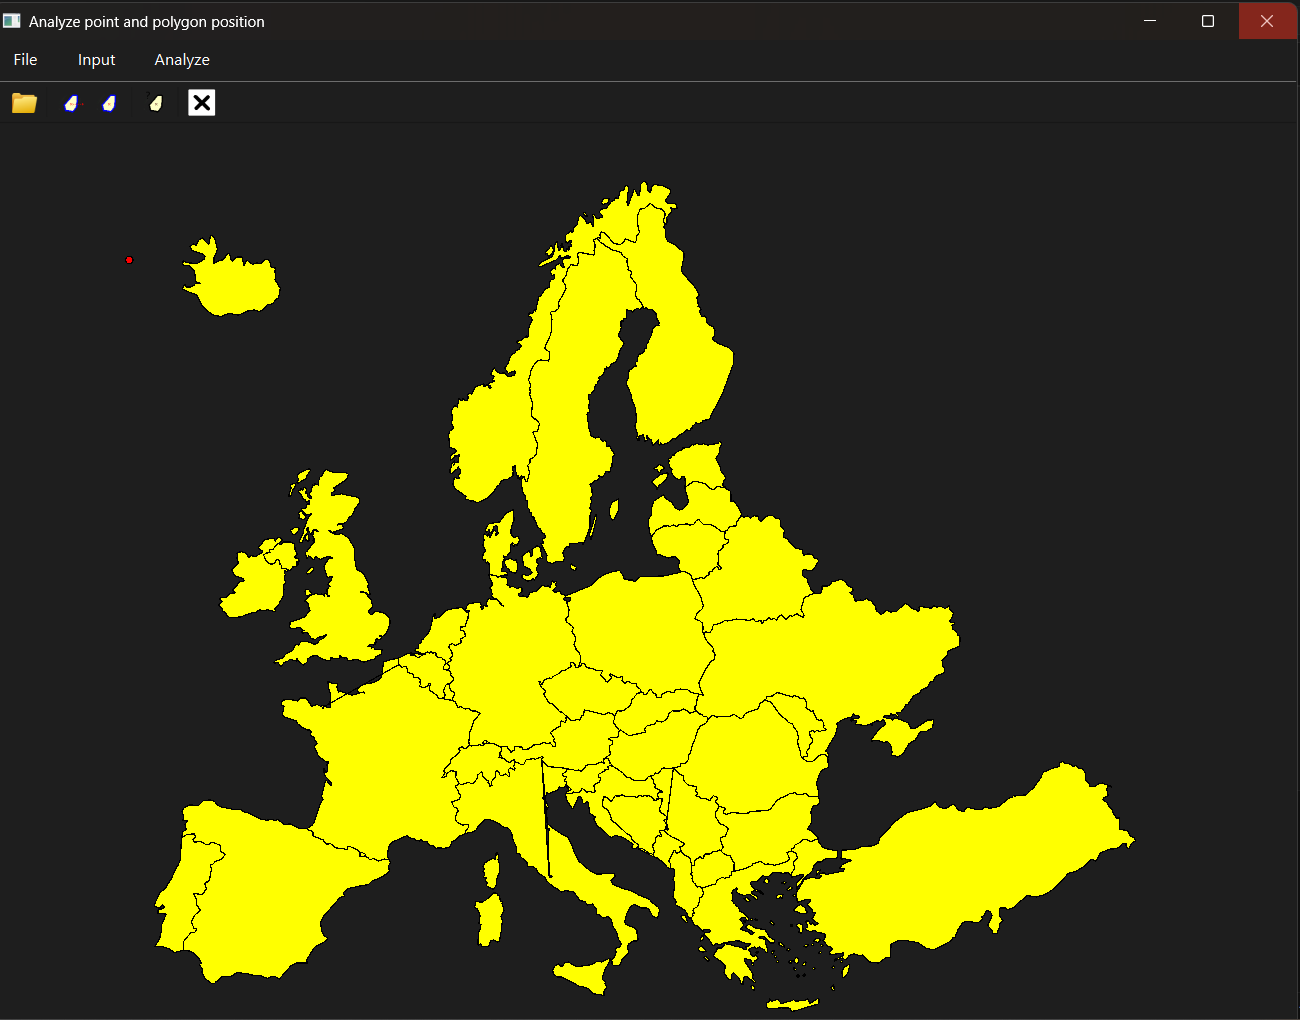
\includegraphics[width=0.9\linewidth]{figures/apka.png}
    \caption{Printscreen vytvořené aplikace s načtenými daty.}
    \label{fig:obr1}
\end{figure}


\newpage
\subsection{Dokumentace}
\subsubsection{Třída Algorithms}
Třída \textit{Algorithms} zahrnuje metody \textit{getBoundingBox}, \textit{getPointPolygonPositionRC} a \textit{getPointPolygonPositionWN}.
První metoda slouží k určení min-max boxu a vrací minima a maxima x-ových a y-ových souřadnic.
Druhá metoda analyzuje vzájemnou polohu polygonu a bodu pomocí Ray Crossing algoritmu a vrací informaci o tom, ve kterém polygonu se bod nachází.
Třetí metoda provádí totožnou analýzu, ale používá k tomu Winding Number algoritmus.

\subsubsection{Třída Draw}
Třída \textit{Draw} obsahuje metody \textit{mousePressEvent} - změna polohy kurzoru myši při kliknutí, \textit{paintEvent} - vykreslení bodu či polygonu, \textit{changeStatus}, \textit{clearData} - vymazání všech polygonů a bodu na obrazovce, \textit{getQ} - vrácení bodu, \textit{getPol} - vrácení polygonů, \textit{setHighlightedPolygon} - zvýraznění polygonu, kterému náleží analyzovaný bod a \textit{LoadShapesToScene} - načtení vstupních dat ve formátu shapefile.

\subsubsection{Třída Main Form}
Třída \textit{Main Form} slouží ke spuštění grafického rozhraní aplikace a propojuje jednotlivé metody definované v ostatních třídách.

\newpage
\subsection{Závěr}
V rámci této  práce byla úspěšně vytvořena aplikace v prostředí QT, která řeší geometrické vyhledávání bodu v polygonu (Point Location Problem). Implementovány byly dva algoritmy: Ray Crossing Algorithm a Winding Number Algorithm.
Oba algoritmy byly upraveny tak, zpracovávaly nejen jednoduché, ale i komplexní polygony s dírami. 
Pro zvýšení výpočetní efektivity byla implementována metoda min-max boxu (Bounding Box), která výrazně urychluje vyhledávání v rozsáhlých datasetech tím, že vylučuje polygony, v jejichž obdélníkovém opsaném celku se bod $q$ nenachází.
Aplikace umožňuje přímé načítání dat ve formátu .shp. Součástí řešení bylo i matematické přemapování souřadnic z geografického systému do souřadnicového systému obrazovky se zachováním aspektu a definovaným okrajem.

Při testování na reálných datech z Eurostatu se u vybraných entit (např. Itálie) projevila grafická chyba v interpretaci polygonu. Jak je patrné z obrázku~\ref{fig:obr2}, pravděpodobnou příčinou je buď nekonzistence ve vstupním shapefilu, nebo specifická chyba při transformaci souřadnicových polí u velmi členitých objektů. Tato anomálie však nemá vliv na matematickou správnost vyhodnocení polohy bodu algoritmy RC a WN.

Námětem na vylepšení by mohlo být vyskakovací okno zobrazující atributová data (název země) při kliknutí.

\begin{figure}[h!]
    \centering
    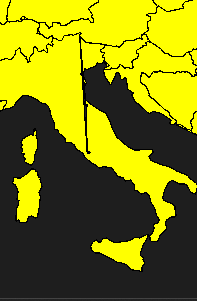
\includegraphics[width=0.3\linewidth]{figures/image.png}
    \caption{Printscreen chyby při načítání shapefile Evropy.}
    \label{fig:obr2}
\end{figure}







